\documentclass[titlepage,11pt]{article}

\textwidth 6.5in
\textheight 9in
\oddsidemargin -0.2in
\topmargin -0.5in

\usepackage{indentfirst,graphics,alltt,epsfig,color}

\title{iBioSim: Installation Instructions}

\author{Chris J. Myers}

\date{Created: August 11th, 2008\\
  Last Revised: August 11th, 2008
}

\begin{document}

\maketitle

%show only subsection granularity in the toc
%\setcounter{tocdepth}{2} 
  
\tableofcontents

\clearpage
  
%\setlength{\parindent}{0em}
%\setlength{\parskip}{10pt}

\section{General Requirements}

\noindent
There are versions of {\tt iBioSim} available for Windows, Linux, and
MacOS.  You can download the appropriate installation file from:\\
{\tt http://www.async.ece.utah.edu/iBioSim}
To install follow the instuctions for your operating system below.

DESCRIBE Java, Graphviz requirements

\section{Installation on Windows}

\noindent
Download and execute {\tt iBioSim-$\langle$version$\rangle$-Setup.exe}.
MORE HERE

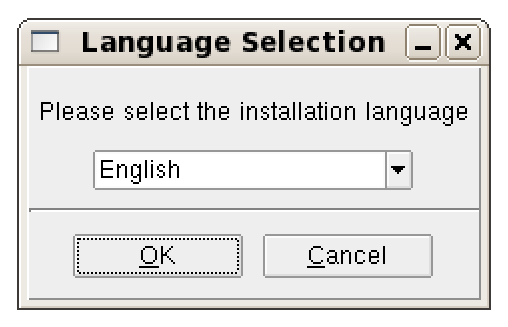
\includegraphics[height=50mm]{screenshots/language}

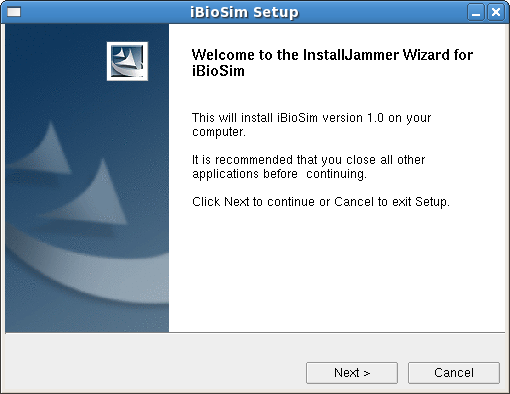
\includegraphics[height=50mm]{screenshots/setup}

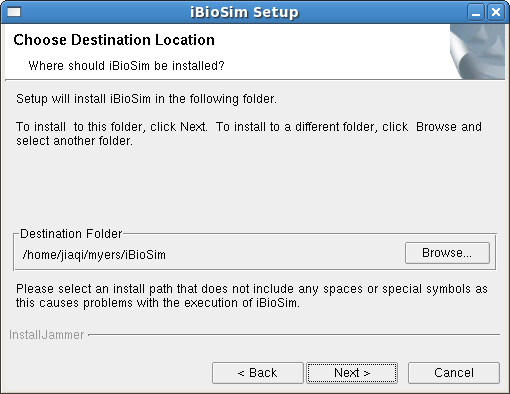
\includegraphics[height=50mm]{screenshots/location}

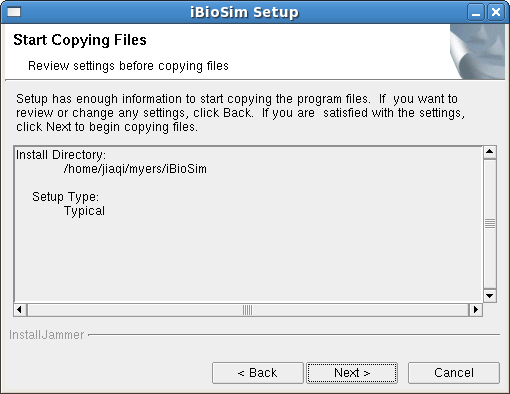
\includegraphics[height=50mm]{screenshots/confirm}

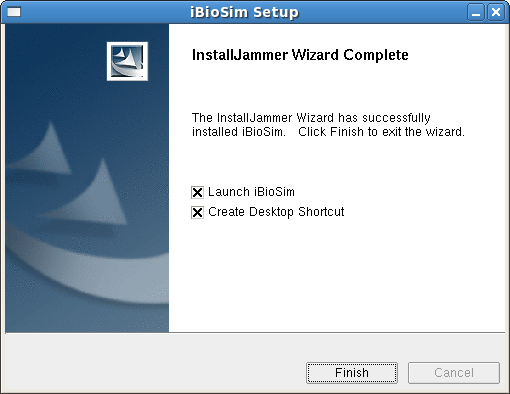
\includegraphics[height=50mm]{screenshots/finish}

EXPLAIN UNINSTALL

\section{Installation on Linux}

\noindent
Download {\tt iBioSim-$\langle$version$\rangle$-Linux-x86-Install}.
Change permissions on this file to allow it to be executed:\\
{\tt chmod u+x iBioSim-$\langle$version$\rangle$-Linux-x86-Install}.
Executing this file will now start the install shield.

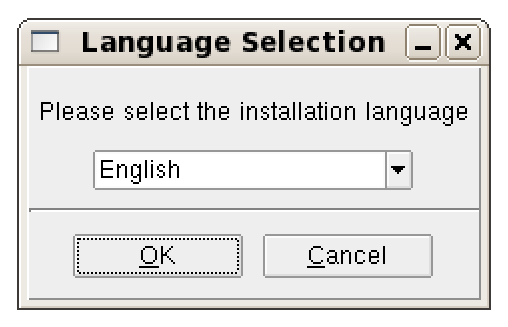
\includegraphics[height=50mm]{screenshots/language}

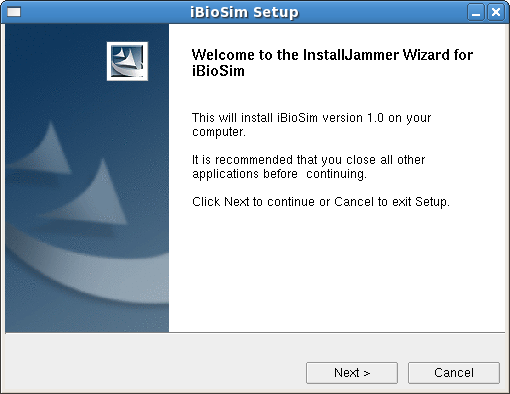
\includegraphics[height=50mm]{screenshots/setup}

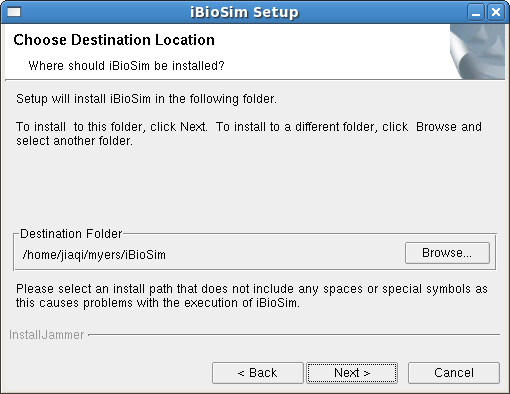
\includegraphics[height=50mm]{screenshots/location}

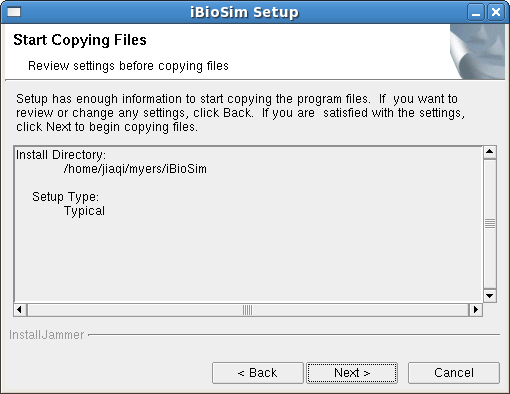
\includegraphics[height=50mm]{screenshots/confirm}

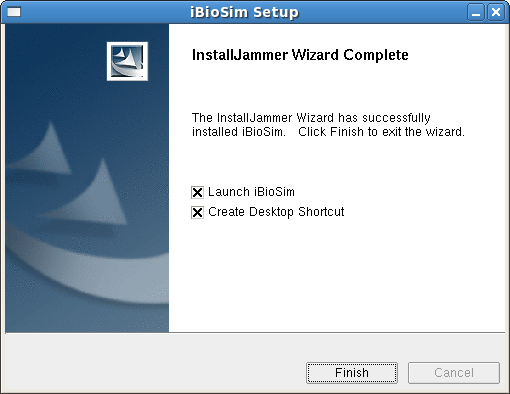
\includegraphics[height=50mm]{screenshots/finish}


EXPLAIN UNINSTALL

\section{Installation on MacOS}

\noindent
EXPLAIN IT HERE

EXPLAIN UNINSTALL

\end{document}
